\documentclass[tikz,border=2pt]{standalone}
\usepackage{amsmath,amssymb}
\usepackage{tikz}
\usetikzlibrary{arrows.meta}

\begin{document}
% Two independent Poisson arrival counts (means 3 and 7) put together: the total count is
% Poisson with mean 10.
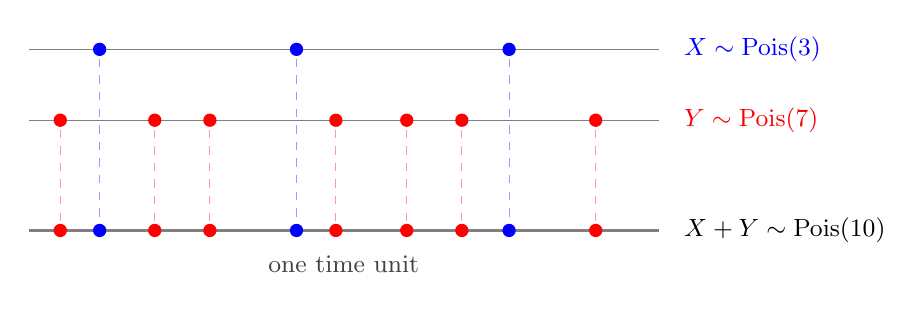
\begin{tikzpicture}[every node/.style={font=\small}, >={Latex[length=2mm]}]
	\draw[gray] (0,0) -- (8,0);
	\draw[gray] (0,-0.9) -- (8,-0.9);
	\draw[gray, thick] (0,-2.3) -- (8,-2.3);
	\foreach \x in {0.9, 3.4, 6.1} {
		\fill[blue] (\x,0) circle (2.4pt);
		\fill[blue] (\x,-2.3) circle (2.4pt);
		\draw[blue!40, dashed] (\x,-0.12) -- (\x,-2.18);
	}
	\foreach \x in {0.4, 1.6, 2.3, 3.9, 4.8, 5.5, 7.2} {
		\fill[red] (\x,-0.9) circle (2.4pt);
		\fill[red] (\x,-2.3) circle (2.4pt);
		\draw[red!40, dashed] (\x,-1.02) -- (\x,-2.18);
	}
	\node[blue, anchor=west] at (8.2,0) {$X\sim\operatorname{Pois}(3)$};
	\node[red, anchor=west] at (8.2,-0.9) {$Y\sim\operatorname{Pois}(7)$};
	\node[anchor=west] at (8.2,-2.3) {$X+Y\sim\operatorname{Pois}(10)$};
	\node[anchor=north, font=\small, gray!50!black] at (4,-2.5) {one time unit};
	
\end{tikzpicture}
\end{document}
